% Auto-generated by export_dashboard_networks_latex.py (nx.to_latex_raw)
% cm_overall_min10 | nodes=14 edges=16
  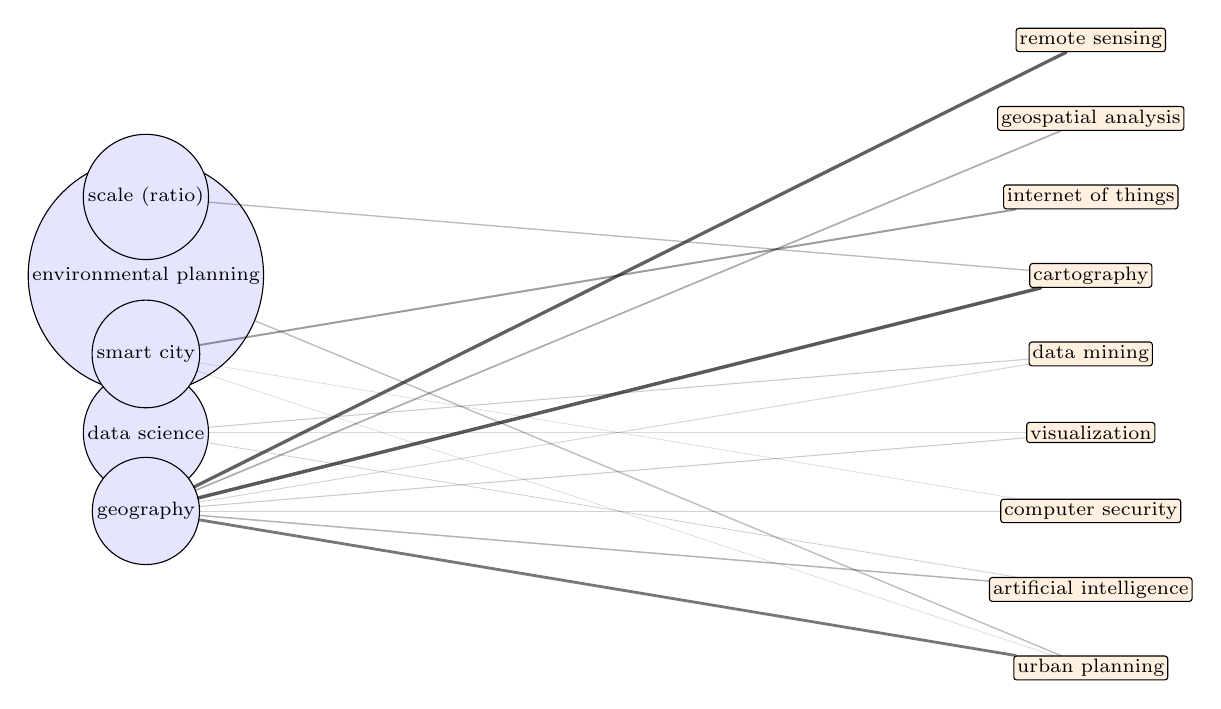
\begin{tikzpicture}[x=1cm,y=1cm,kw/.style={draw,circle,inner sep=1.2pt,font=\scriptsize,fill=black!5},concept/.style={draw,circle,inner sep=1.2pt,font=\scriptsize,fill=blue!10},method/.style={draw,rounded corners=1pt,rectangle,inner sep=1.2pt,font=\scriptsize,fill=orange!12}]
      \draw
        (-6.0, -0.997) node[concept] (n0){data science}
        (6.0, -3.988) node[method] (n1){urban planning}
        (-6.0, 0.997) node[concept] (n2){environmental planning}
        (-6.0, 0.0) node[concept] (n3){smart city}
        (-6.0, -1.994) node[concept] (n4){geography}
        (6.0, -2.991) node[method] (n5){artificial intelligence}
        (6.0, 1.994) node[method] (n6){internet of things}
        (6.0, -1.994) node[method] (n7){computer security}
        (6.0, 2.991) node[method] (n8){geospatial analysis}
        (6.0, 3.988) node[method] (n9){remote sensing}
        (6.0, -0.997) node[method] (n10){visualization}
        (6.0, 0.0) node[method] (n11){data mining}
        (6.0, 0.997) node[method] (n12){cartography}
        (-6.0, 1.994) node[concept] (n13){scale (ratio)};
      \begin{scope}[-,line cap=round]
        \draw[line width=0.309pt,opacity=0.179] (n0) to (n5);
        \draw[line width=0.250pt,opacity=0.150] (n0) to (n10);
        \draw[line width=0.368pt,opacity=0.209] (n0) to (n11);
        \draw[line width=0.485pt,opacity=0.268] (n1) to (n2);
        \draw[line width=0.250pt,opacity=0.150] (n1) to (n3);
        \draw[line width=1.015pt,opacity=0.532] (n1) to (n4);
        \draw[line width=0.721pt,opacity=0.385] (n3) to (n6);
        \draw[line width=0.250pt,opacity=0.150] (n3) to (n7);
        \draw[line width=0.309pt,opacity=0.179] (n4) to (n7);
        \draw[line width=0.603pt,opacity=0.326] (n4) to (n8);
        \draw[line width=1.191pt,opacity=0.621] (n4) to (n9);
        \draw[line width=0.368pt,opacity=0.209] (n4) to (n10);
        \draw[line width=0.309pt,opacity=0.179] (n4) to (n11);
        \draw[line width=1.250pt,opacity=0.650] (n4) to (n12);
        \draw[line width=0.544pt,opacity=0.297] (n4) to (n5);
        \draw[line width=0.485pt,opacity=0.268] (n12) to (n13);
      \end{scope}
    \end{tikzpicture}
